\section{Governing equations for ideal fluid flow}
\subsection{The continuity equation for incompressible flow}\label{section:CONTINUITY}
The idealised fluid in this essay is incompressible. This means that if $\rho$ represents the density of the fluid, then as per definition \ref{definition:INCOMPRESSIBLE}, $\rho$ must 
remain constant over time at every point in the domain of the vector field representing the fluid flow. This means that for any arbitrary closed volume within the fluid, the net mass
flow rate across its boundaries must be zero.

Let the velocity vector field of the fluid be $\mathbf{V}:x,y\mapsto X(x,y)\ihat+Y(x,y)\jhat$. To quantify the mass flow, consider an arbitrary infinitesimal rectangular volume within
the fluid, with vertices $W(\alpha_0,\beta_0)$, $X(\alpha_1,\beta_0)$, $Y(\alpha_1,\beta_1)$, and $Z(\alpha_0,\beta_1)$, as depicted below. Let $\bar{\alpha}=\frac{\alpha_0+\alpha_1}{2}$
and $\bar{\beta}=\frac{\beta_0+\beta_1}{2}$. Assume $\mathbf{V}$ is continuous and differentiable over this region.

\begin{center}
    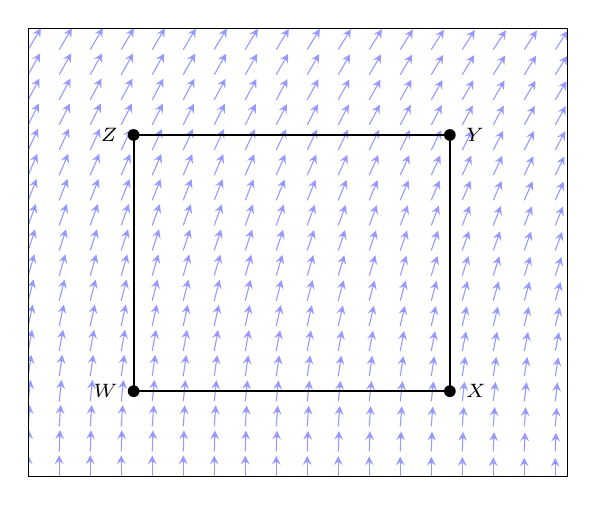
\begin{tikzpicture}[scale=1,X/.style = {circle, fill=black, inner sep=1.5pt,
            label={[font=\scriptsize]left:#1},
            node contents={}},Y/.style = {circle, fill=black, inner sep=1.5pt,
            label={[font=\scriptsize]right:#1},
            node contents={}}]
        \begin{axis}
        [
            domain=0:0.5,
            view={0}{90},
            xtick=\empty,
            ytick=\empty
        ]
        \addplot3[blue, opacity=0.4, quiver={u={sin(deg(y))}, v={cos(deg(x))}, scale arrows=0.025}, -stealth,samples=18] {0};
        \draw[draw=black, thick] (0.1,0.1) rectangle ++(0.3,0.3);
        \draw (0.1,0.1) node[X={$W$}];
        \draw (0.4,0.1) node[Y={$X$}];
        \draw (0.4,0.4) node[Y={$Y$}];
        \draw (0.1,0.4) node[X={$Z$}];
        \end{axis}
    \end{tikzpicture}
\end{center}

The mass flow rate ($\dot{m}$, mass per unit time) across a given surface is defined as the flux of mass, which is computed as the product of density, the velocity component normal to the
surface, and the area of the surface. Thus along the $x$ axis (in the direction of $\ihat$) the mass flow rate into $WZ$ is given as,
$$
    \dot{m}_{\rightarrow WZ}=\rho X(\alpha_0,\bar{\beta})(\beta_1-\beta_0)
$$
and similarly the mass flow rate out of the opposite side $XY$ is given as:
$$
    \dot{m}_{XY\rightarrow}=\rho X(\alpha_1,\bar{\beta})(\beta_1-\beta_0)
$$
Thus, the net mass flow rate out of the rectangular region along the $x$ axis is:
\begin{align*}
    \dot{m}_{\ihat}&=\dot{m}_{XY\rightarrow}-\dot{m}_{\rightarrow WZ}\\
    &=\rho X(\alpha_1,\bar{\beta})(\beta_1-\beta_0)-\rho X(\alpha_0,\bar{\beta})(\beta_1-\beta_0)
\end{align*}
Which, factoring out $\rho(\beta_1-\beta_0)$, leads to:
$$
    \dot{m}_{\ihat}=\rho(\beta_1-\beta_0)\left[X(\alpha_1,\bar{\beta})-X(\alpha_0,\bar{\beta})\right]
$$
Analogously, across the $y$ axis, the net mass flow rate out of the rectangular region between sides $WX$ and $ZY$ is given by the expression:
$$
    \dot{m}_{\jhat}=\rho(\alpha_1-\alpha_0)\left[Y(\bar{\alpha},\beta_1)-Y(\bar{\alpha},\beta_0)\right]
$$
Therefore, the net mass flow rate out of the rectangular region, which must be equal to 0 for the fluid to incompressible, is given by:
\begin{align*}
    \dot{m}&=\dot{m}_{\ihat}+\dot{m}_{\jhat}\\
    &=\rho(\beta_1-\beta_0)\left[X(\alpha_1,\bar{\beta})-X(\alpha_0,\bar{\beta})\right]+\rho(\alpha_1-\alpha_0)\left[Y(\bar{\alpha},\beta_1)-Y(\bar{\alpha},\beta_0)\right]=0
\end{align*}
Dividing through by $\rho$, $(\alpha_1-\alpha_0)$ and $(\beta_1-\beta_0)$:
$$
    \frac{X(\alpha_1,\bar{\beta})-X(\alpha_0,\bar{\beta})}{\alpha_1-\alpha_0}+\frac{Y(\bar{\alpha},\beta_1)-Y(\bar{\alpha},\beta_0)}{\beta_1-\beta_0}=0
$$
Now consider the limit as $\alpha_1\rightarrow\alpha_0$ and $\beta_1\rightarrow\beta_0$, the difference $\delta_\alpha=\alpha_1-\alpha_0\rightarrow0$ and $\delta_\beta=\beta_1-\beta_0\rightarrow0$.
\begin{align*}
    \lim_{\delta_\alpha\rightarrow0}\frac{X(\alpha_0+\delta_\alpha,\bar{\beta})-X(\alpha_0,\bar{\beta})}{\delta_\alpha}&=\eval{\pdv{X}{x}}_{\point{\alpha_0}{\bar{\beta}}}\\
    \lim_{\delta_\beta\rightarrow0}\frac{Y(\bar{\alpha},\beta_0+\delta_\beta)-Y(\bar{\alpha},\beta_0)}{\delta_\beta}&=\eval{\pdv{Y}{y}}_{\point{\bar{\alpha}}{\beta_0}}
\end{align*}
Furthermore, as $\alpha_1\rightarrow\alpha_0$ and $\beta_1\rightarrow\beta_0$, $\bar{\alpha}\rightarrow\alpha_0$ and $\bar{\beta}\rightarrow\beta_0$, consequently
$$
    \dot{m}=\eval{\pdv{X}{x}}_{\point{\alpha_0}{\beta_0}}+\eval{\pdv{Y}{y}}_{\point{\alpha_0}{\beta_0}}=\eval{\divergence{\mathbf{V}}}_{\point{\alpha_0}{\beta_0}}=0
$$
Because $\point{\alpha_0}{\beta_0}$ is any point in the domain of $\mathbf{V}$ where the function is differentiable, the expression can be generalised as
$$
    \divergence{\mathbf{V}}=0
$$
This equation is known as the continuity equation for incompressible fluids \cite{PHAM2014405} and will underpin following derivations made in this essay.

\subsection{Irrotational flow}\label{section:IRROTATIONAL}
As mentioned in definition \ref{definition:VP}, one resulting property of the idealisations (steady, inviscid and incompressible flow)
made in this essay is irrotational flow. If flow is rotational, then there exists points at which $\curl{\fatf}\neq0$. In other words, if one were to
imagine a water wheel at some point in the fluid, and it spins, then the flow is rotational, and vice versa for irrotational flow.
However, flow being irrotational does not imply that it cannot curve, for example $\curl{\fatf}=0$ in cases such as:
\begin{align*}
    &\fatf:x,y\mapsto X(x,y)\ihat+Y(x,y)\jhat\quad\forall\point{x}{y}\neq\point{0}{0}\\
    &X:x,y\mapsto-\frac{y}{x^2+y^2}\,,\quad Y:x,y\mapsto\frac{x}{x^2+y^2}
\end{align*}
Applying the quotient rule to compute the derivatives for both $X$ and $Y$ gives:
\begin{align*}
    \pdv{X}{y}&=-\frac{\left(\pdv{y}y\right)\left(x^2+y^2\right)-y\pdv{y}\left(x^2+y^2\right)}{\left(x^2+y^2\right)^2}\\
    &=-\frac{x^2+y^2-y(2y)}{\left(x^2+y^2\right)^2}\\
    &=-\frac{x^2-y^2}{\left(x^2+y^2\right)^2}
\end{align*}
\begin{align*}
    \pdv{Y}{x}&=\frac{\left(\pdv{x}x\right)\left(x^2+y^2\right)-x\pdv{x}\left(x^2+y^2\right)}{\left(x^2+y^2\right)^2}\\
    &=\frac{x^2+y^2-x(2x)}{\left(x^2+y^2\right)^2}\\
    &=\frac{-x^2+y^2}{\left(x^2+y^2\right)^2}=-\frac{x^2-y^2}{\left(x^2+y^2\right)^2}
\end{align*}
Thus,
\begin{align*}
    \pdv{X}{y}=\pdv{Y}{x}\implies\pdv{Y}{x}-\pdv{X}{y}=0\\
    \therefore\curl{\fatf}=0
\end{align*}
Plotting the vector field for $\fatf$ reveals circulation around the origin, suggesting rotational flow, but which, with a curl of 0 (everywhere except for
the origin, where $\fatf$ is undefined), is irrotational\referto{figure}{figure:ZEROCURL}.
\begin{figure*}[!ht]
    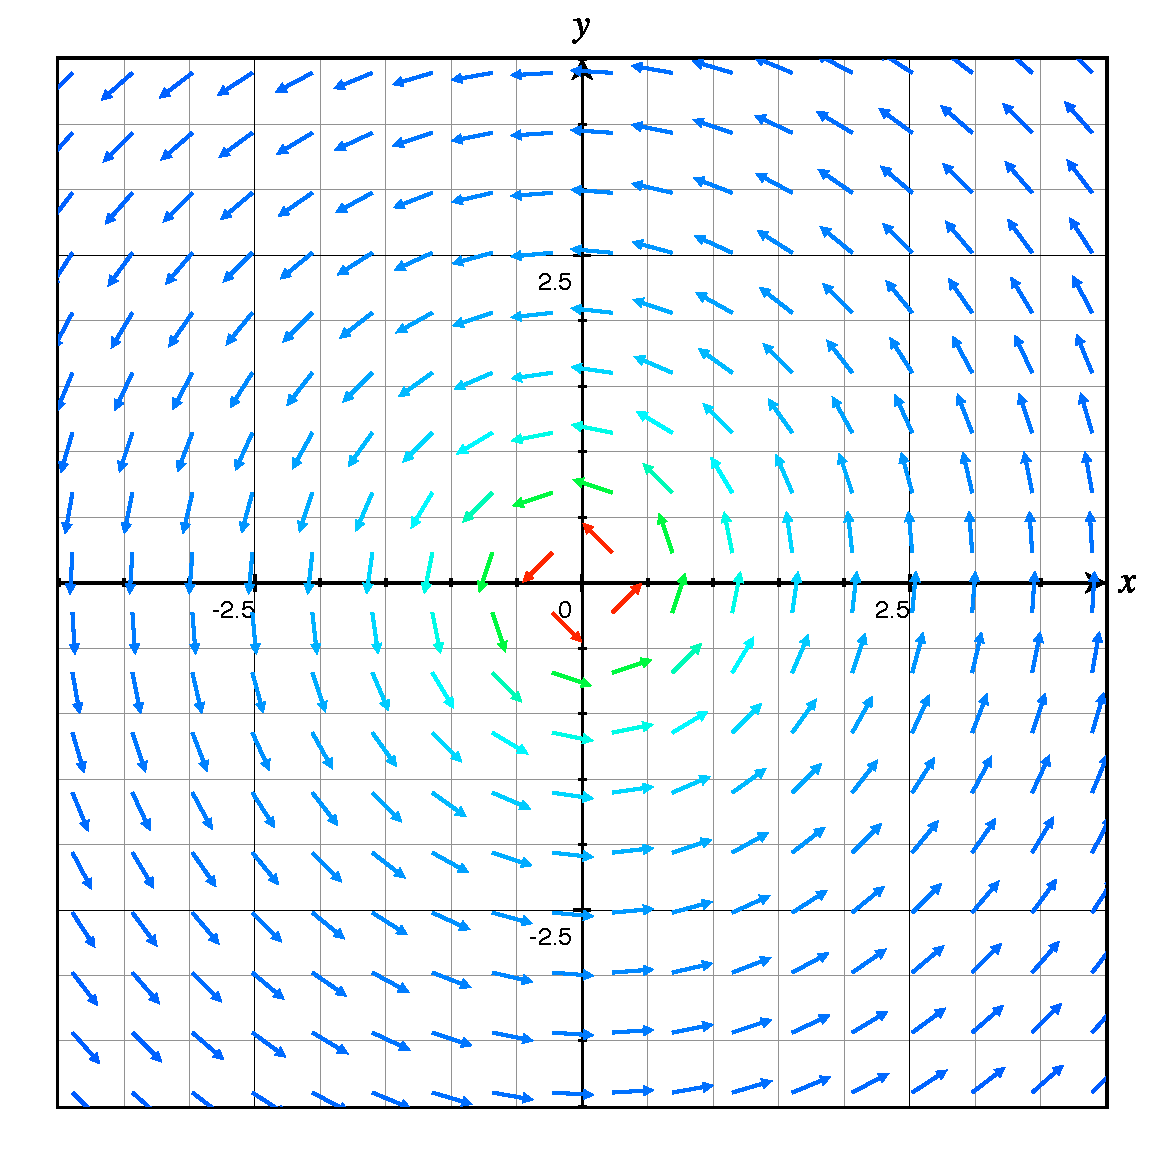
\includegraphics[scale=0.5]{0_curl.pdf}
    \centering
    \caption{The function $\fatf:x,y\mapsto\begin{pmatrix}
        -y\left(x^2+y^2\right)^{-1}\\x\left(x^2+y^2\right)^{-1}
    \end{pmatrix}$ is irrotational despite curving}
    \label{figure:ZEROCURL}
\end{figure*}

% KELVINS THEOREM

\newpage % temporary formatting solution
\subsection{The velocity potential}\label{section:POTENTIAL}
As established in Section~\ref{section:IRROTATIONAL}, for an incompressible and inviscid fluid initially irrotational, the flow remains irrotational, meaning
the velocity field $\vec{V}$ modelling the flow satisfies $\curl{\vec{V}}=0$. This condition leads to the existence of a scalar-valued function, known as the
velocity potential, whose gradient is equal to the vector field. To demonstrate this, consider the identity $\curl{\gradient{\phi}}$, where $\phi$ is a
function of $x$ and $y$ and is scalar valued. $\gradient{\phi}$ is defined as:
$$
    \gradient{\phi}=\begin{bmatrix}
        \pdv*{\phi}{x}\\
        \pdv*{\phi}{y}
    \end{bmatrix}
$$
Taking the curl of this expression and applying Theorem~\ref{lemma:CLAIRAUT} (Clairaut's theorem) gives
\begin{align*}
    \curl{\gradient{\phi}}&=\pdv{\phi}{y}{x}-\pdv{\phi}{x}{y}\\
                             &=\pdv{\phi}{y}{x}-\pdv{\phi}{y}{x}=0
\end{align*}
Thus, by the definition of irrotational flow,
\begin{align*}
    \curl{\vec{V}}&=0=\curl{\gradient{\phi}}\\
    \therefore\vec{V}&=\gradient{\phi}
\end{align*}
Here, $\phi$ is known as the velocity potential of $\vec{V}$. The velocity potential makes derivations made in this essay easier due its scalar valued nature.

\subsection{The multivariable chain rule}
\subsubsection{The Jacobian matrix}
\begin{defn}
    The \definedterm{Jacobian matrix} of some function $\fatf$, denoted $\jacobian_\fatf$, is defined as the matrix containing all the first order partial derivatives
    of the function. For the function
    $$\fatf:x_1,x_2,\cdots,x_n\mapsto\begin{bmatrix}
        f_1(x_1,x_2,\cdots,x_n)\\
        f_2(x_1,x_2,\cdots,x_n)\\
        \vdots\\
        f_m(x_1,x_2,\cdots,x_n)
    \end{bmatrix}$$
    the Jacobian of $\fatf$ would be given as
    $$
        \jacobian_\fatf=\begin{bmatrix}
            \nabla^\top f_1\\
            \nabla^\top f_2\\
            \vdots\\
            \nabla^\top f_m
        \end{bmatrix}=\begin{bmatrix}
            \pdv*{f_1}{x_1} & \pdv*{f_1}{x_2} & \cdots & \pdv*{f_1}{x_n}\\
            \pdv*{f_2}{x_1} & \pdv*{f_2}{x_2} & \cdots & \pdv*{f_2}{x_n}\\
            \vdots & \vdots & \ddots & \vdots \\
            \pdv*{f_m}{x_1} & \pdv*{f_m}{x_2} & \cdots & \pdv*{f_m}{x_n}\\
        \end{bmatrix}\in\mathbb{R}^{m\times n}
    $$
\end{defn}
The Jacobian matrix, and its determinant, has many uses within vector calculus, but for the purposes of this essay, the Jacobian chain rule is a fundamental result which allows for the calculation of the derivatives of a composite functions. The following result and proof underpins the proof for the more generalised version in Section~\ref{section:MVCR}.
\begin{lemma}[The Jacobian chain rule]\label{lemma:JACOBIAN-CHAIN}
    Let the function $\fatf:\mathbb{R}^m\rightarrow\mathbb{R}^n$ and the function $\vec{G}:\mathbb{R}^l\rightarrow\mathbb{R}^m$. The Jacobian of the composite
    $\fatf\circ\vec{G}$ evaluated at some point $\vec{p}$ can be expressed as
    $$
        \jacobian_{\fatf\circ\vec{G}}(\vec{p})=\left[\jacobian_\fatf\circ\vec{G}(\vec{p})\right]\jacobian_\vec{G}(\vec{p})
    $$
    \begin{proof}
        A function $\fatf:\mathbb{R}^m\rightarrow\mathbb{R}^n$ is considered differentiable at some point $\vec{a}$ if there exists a linear map such (represented by its
        Jacobian matrix $\jacobian_\fatf(\vec{a})$)that for an infinitesimal vector $\vec{h}$
        $$
            \fatf(\vec{a}+\vec{h})-\fatf(\vec{a})=\jacobian_\fatf(\vec{a})\vec{h}+\epsilon(\vec{h})
        $$
        where $\epsilon(\vec{h})$ is an error term such that it vanishes faster than the magnitude of $\vec{h}$:
        \begin{equation}
            \label{equation:ERROR}\lim_{\vec{h}\rightarrow\vec{0}}\frac{\lVert\epsilon(\vec{h})\rVert}{\lVert\vec{h}\rVert}=\vec{0}
        \end{equation}
        Consider the function $\vec{Z}:\vec{t}\mapsto(\fatf\circ \vec{G})(\vec{t})$, where $\vec{G}:\mathbb{R}^l\rightarrow\mathbb{R}^m$ and $\fatf:\mathbb{R}^m\rightarrow\mathbb{R}^n$. For
        some small change in $\vec{t}$, called $\delta_\vec{t}$, the change in the inner function $\vec{G}$ can be expressed using its differentiability at $\vec{t}$
        \begin{equation}
            \label{equation:jacobian-chain-rule:1}\delta_\vec{G}=\vec{G}(\vec{t}+\delta_\vec{t})-\vec{G}(t)=\jacobian_\vec{G}(\vec{t})\delta_\vec{t}+\epsilon_\vec{G}(\delta_\vec{t})
        \end{equation}
        The error term $\epsilon_\vec{G}(\delta_t)$ satisfies \eqref{equation:ERROR}. Then consider the change of the outer function $\fatf$, also expressed using its differentiability
        at the point $\vec{u}=\vec{G}(\vec{t})$,
        $$
            \delta_\fatf=\fatf(\vec{u}+\delta_\vec{G})-\fatf(\vec{u})=\jacobian_\fatf(\vec{u})\delta_\vec{G}+\epsilon_\fatf(\delta_\vec{G})
        $$
        Which, since $\vec{Z}=(\fatf\circ\vec{G})(\vec{t})$, means that
        \begin{equation}
            \label{equation:jacobian-chain-rule:2}\delta_\vec{Z}=\delta_\fatf=\fatf(\vec{u}+\delta_\vec{G})-\fatf(\vec{u})=\jacobian_\fatf(\vec{u})\delta_\vec{G}+\epsilon_\fatf(\delta_\vec{G})
        \end{equation}
        Let the error term $\epsilon_\fatf(\delta_\vec{G})$ also satisfy \eqref{equation:ERROR}. Then, substituting \eqref{equation:jacobian-chain-rule:1} into \eqref{equation:jacobian-chain-rule:2},
        \begin{align*}
            \delta_\vec{Z}&=\jacobian_\fatf(\vec{u})\left[\jacobian_\vec{G}(\vec{t})\delta_\vec{t}+\epsilon_\vec{G}(\delta_\vec{t})\right]+\epsilon_\fatf(\jacobian_\vec{G}(\vec{t})\delta_\vec{t}+\epsilon_\vec{G}(\delta_\vec{t}))\\
            &=\jacobian_\fatf(\vec{u})\jacobian_\vec{G}(\vec{t})\delta_\vec{t}+\jacobian_\fatf(\vec{u})\epsilon_\vec{G}(\delta_\vec{t})+\epsilon_\fatf(\jacobian_\vec{G}(\vec{t})\delta_\vec{t}+\epsilon_\vec{G}(\delta_\vec{t}))
        \end{align*}
        Dividing through by $\lVert\delta_\vec{t}\rVert$,
        $$
            \frac{\delta_\vec{Z}}{\lVert\delta_\vec{t}\rVert}=\jacobian_\fatf(\vec{u})\jacobian_\vec{G}(\vec{t})\overbrace{\frac{\delta_\vec{t}}{\lVert\delta_\vec{t}\rVert}}^{\text{\makebox[0pt]{Henceforth $\hat{\delta_\vec{t}}$}}}+\jacobian_\fatf(\vec{u})\frac{\epsilon_\vec{G}(\delta_\vec{t})}{\lVert\delta_\vec{t}\rVert}+\frac{\epsilon_\fatf(\jacobian_\vec{G}(\vec{t})\delta_\vec{t}+\epsilon_\vec{G}(\delta_\vec{t}))}{\lVert\delta_\vec{t}\rVert}
        $$
        Considering the value of the error terms as $\delta_\vec{t}\rightarrow\vec{0}$,
        $$
            \lim_{\delta_\vec{t}\rightarrow\vec{0}}\jacobian_\fatf(\vec{u})\frac{\epsilon_\vec{G}(\delta_\vec{t})}{\lVert\delta_\vec{t}\rVert}+\frac{\epsilon_\fatf(\jacobian_\vec{G}(\vec{t})\delta_\vec{t}+\epsilon_\vec{G}(\delta_\vec{t}))}{\lVert\delta_\vec{t}\rVert}
        $$
        For any matrix $\vec{M}$ and vector $\vec{v}$, the magnitude of their product $\lVert\vec{M}\vec{v}\rVert\leq\lVert\vec{M}\rVert\lVert\vec{v}\rVert$, thus for the first term,
        \begin{align*}
            \lim_{\delta_\vec{t}\rightarrow\vec{0}}\lVert\jacobian_\fatf(\vec{u})\frac{\epsilon_\vec{G}(\delta_\vec{t})}{\lVert\delta_\vec{t}\rVert}\rVert&\leq\lim_{\delta_\vec{t}\rightarrow\vec{0}}\lVert\jacobian_\fatf(\vec{u})\rVert\lVert\frac{\epsilon_\vec{G}(\delta_\vec{t})}{\lVert\delta_\vec{t}\rVert}\rVert\\
            &=\lim_{\delta_\vec{t}\rightarrow\vec{0}}\lVert\jacobian_\fatf(\vec{u})\rVert\frac{\lVert\epsilon_\vec{G}(\delta_\vec{t})\rVert}{\lVert\delta_\vec{t}\rVert}
        \end{align*}
        By the definition of the definition of the error term $\lim_{\delta_\vec{t}\rightarrow\vec{0}}\frac{\lVert\epsilon_\vec{G}(\delta_\vec{t})\rVert}{\lVert\delta_\vec{t}\rVert}=0$, therefore
        \begin{align*}
            \lim_{\delta_\vec{t}\rightarrow\vec{0}}\lVert\jacobian_\fatf(\vec{u})\frac{\epsilon_\vec{G}(\delta_\vec{t})}{\lVert\delta_\vec{t}\rVert}\rVert&\leq\lim_{\delta_\vec{t}\rightarrow\vec{0}}\lVert\jacobian_\fatf(\vec{u})\rVert\frac{\lVert\epsilon_\vec{G}(\delta_\vec{t})\rVert}{\lVert\delta_\vec{t}\rVert}\\
            \implies\lim_{\delta_\vec{t}\rightarrow\vec{0}}\lVert\jacobian_\fatf(\vec{u})\frac{\epsilon_\vec{G}(\delta_\vec{t})}{\lVert\delta_\vec{t}\rVert}\rVert&\leq0\\
            \therefore\lim_{\delta_\vec{t}\rightarrow\vec{0}}\lVert\jacobian_\fatf(\vec{u})\frac{\epsilon_\vec{G}(\delta_\vec{t})}{\lVert\delta_\vec{t}\rVert}\rVert&=0\implies\lim_{\delta_\vec{t}\rightarrow\vec{0}}\jacobian_\fatf(\vec{u})\frac{\epsilon_\vec{G}(\delta_\vec{t})}{\lVert\delta_\vec{t}\rVert}=\vec{0}
        \end{align*}
        % For the second error term, consider the value of the input of $\epsilon_\fatf$ as $\delta_\vec{t}\rightarrow\vec{0}$
        % $$
        %     \lim_{\delta_\vec{t}\rightarrow\vec{0}}\underbrace{\jacobian_\vec{G}(\vec{t})\delta_\vec{t}}_{\text{Term }\alpha}+\underbrace{\epsilon_\vec{G}(\delta_\vec{t})}_{\text{Term }\beta}
        % $$
        % For term $\alpha$, apply the same logic as for the previous error term
        % \begin{align*}
        %     \lim_{\delta_\vec{t}\rightarrow\vec{0}}\lVert\jacobian_\vec{G}(\vec{t})\delta_\vec{t}\rVert&\leq\lim_{\delta_\vec{t}\rightarrow\vec{0}}\lVert\jacobian_\vec{G}(\vec{t})\rVert\lVert\delta_\vec{t}\rVert=0\\
        %     \therefore\lim_{\delta_\vec{t}\rightarrow\vec{0}}\jacobian_\vec{G}(\vec{t})\delta_\vec{t}&=\vec{0}
        % \end{align*}
        % For term $\beta$, by definition,
        % \begin{align*}
        %     \lim_{\delta_\vec{t}\rightarrow\vec{0}}\lVert\epsilon_\vec{G}(\delta_\vec{t})\rVert&=0\\
        %     \therefore\lim_{\delta_\vec{t}\rightarrow\vec{0}}\epsilon_\vec{G}(\delta_\vec{t})=\vec{0}
        % \end{align*}
        The second error term can be shown to also be equal to $\vec{0}$ through rearrangment,
        \begin{align*}
            \lim_{\delta_\vec{t}\rightarrow\vec{0}}\frac{\epsilon_\fatf(\jacobian_\vec{G}(\vec{t})\delta_\vec{t}+\epsilon_\vec{G}(\delta_\vec{t}))}{\lVert\delta_\vec{t}\rVert}&=\lim_{\delta_\vec{t}\rightarrow\vec{0}}\frac{\epsilon_\fatf(\jacobian_\vec{G}(\vec{t})\delta_\vec{t}+\epsilon_\vec{G}(\delta_\vec{t}))}{\lVert\jacobian_\vec{G}(\vec{t})\delta_\vec{t}+\epsilon_\vec{G}(\delta_\vec{t})\rVert}\frac{\lVert\jacobian_\vec{G}(\vec{t})\delta_\vec{t}+\epsilon_\vec{G}(\delta_\vec{t})\rVert}{\lVert\delta_\vec{t}\rVert}\\
            &=\lim_{\delta_\vec{t}\rightarrow\vec{0}}\frac{\epsilon_\fatf(\jacobian_\vec{G}(\vec{t})\delta_\vec{t}+\epsilon_\vec{G}(\delta_\vec{t}))}{\lVert\jacobian_\vec{G}(\vec{t})\delta_\vec{t}+\epsilon_\vec{G}(\delta_\vec{t})\rVert}\lim_{\delta_\vec{t}\rightarrow\vec{0}}\frac{\lVert\jacobian_\vec{G}(\vec{t})\delta_\vec{t}+\epsilon_\vec{G}(\delta_\vec{t})\rVert}{\lVert\delta_\vec{t}\rVert}\\
            &=\vec{0}\lim_{\delta_\vec{t}\rightarrow\vec{0}}\frac{\lVert\jacobian_\vec{G}(\vec{t})\delta_\vec{t}+\epsilon_\vec{G}(\delta_\vec{t})\rVert}{\lVert\delta_\vec{t}\rVert}\\
            \lim_{\delta_\vec{t}\rightarrow\vec{0}}\frac{\lVert\jacobian_\vec{G}(\vec{t})\delta_\vec{t}+\epsilon_\vec{G}(\delta_\vec{t})\rVert}{\lVert\delta_\vec{t}\rVert}&\leq\lim_{\delta_\vec{t}\rightarrow\vec{0}}\frac{\lVert\jacobian_\vec{G}(\vec{t})\delta_\vec{t}\rVert}{\lVert\delta_\vec{t}\rVert}+\frac{\lVert\epsilon_\vec{G}(\delta_\vec{t})\rVert}{\lVert\delta_\vec{t}\rVert}\\
            &=\lim_{\delta_\vec{t}\rightarrow\vec{0}}\frac{\lVert\jacobian_\vec{G}(\vec{t})\delta_\vec{t}\rVert}{\lVert\delta_\vec{t}\rVert}+\vec{0}\leq\lim_{\delta_\vec{t}\rightarrow\vec{0}}\frac{\lVert\jacobian_\vec{G}(\vec{t})\rVert\lVert\delta_\vec{t}\rVert}{\lVert\delta_\vec{t}\rVert}+\vec{0}\\
            &=\lVert\jacobian_\vec{G}(\vec{t})\rVert\\
            \therefore\lim_{\delta_\vec{t}\rightarrow\vec{0}}\frac{\epsilon_\fatf(\jacobian_\vec{G}(\vec{t})\delta_\vec{t}+\epsilon_\vec{G}(\delta_\vec{t}))}{\lVert\delta_\vec{t}\rVert}&\leq\vec{0}\lVert\jacobian_\vec{G}(\vec{t})\rVert=\vec{0}\,\forall\lVert\jacobian_\vec{G}(\vec{t})\rVert\\
            \therefore\lim_{\delta_\vec{t}\rightarrow\vec{0}}\frac{\epsilon_\fatf(\jacobian_\vec{G}(\vec{t})\delta_\vec{t}+\epsilon_\vec{G}(\delta_\vec{t}))}{\lVert\delta_\vec{t}\rVert}&=\vec{0}
        \end{align*}
        Thus, both of the error terms approach $\vec{0}$, meaning that
        \begin{align}
            \notag\lim_{\delta_\vec{t}\rightarrow\vec{0}}\frac{\delta_\vec{Z}}{\lVert\delta_\vec{t}\rVert}&=\lim_{\delta_\vec{t}\rightarrow0}\jacobian_\fatf(\vec{u})\jacobian_\vec{G}(\vec{t})\hat{\delta_\vec{t}}+\jacobian_\fatf(\vec{u})\frac{\epsilon_\vec{G}(\delta_\vec{t})}{\lVert\delta_\vec{t}\rVert}+\frac{\epsilon_\fatf(\jacobian_\vec{G}(\vec{t})\delta_\vec{t}+\epsilon_\vec{G}(\delta_\vec{t}))}{\lVert\delta_\vec{t}\rVert}\\
            \notag&=\lim_{\delta_t\rightarrow0}\jacobian_\fatf(\vec{u})\jacobian_\vec{G}(\vec{t})\hat{\delta_\vec{t}}+\vec{0}+\vec{0}\\
            \label{equation:jacobian-chain-rule:3}&=\jacobian_\fatf(\vec{G}(\vec{t}))\jacobian_\vec{G}(\vec{t})\hat{\delta_\vec{t}}=\left[\jacobian_\fatf\circ\vec{G}(\vec{t})\right]\jacobian_\vec{G}(\vec{t})\hat{\delta_\vec{t}}
        \end{align}
        Using the definition of differentiability again for $\vec{Z}$ at $\vec{t}$,
        \begin{align}
            \notag\delta_\vec{Z}&=\vec{Z}(\vec{t}+\delta_\vec{t})-\vec{Z}(\vec{t})=\jacobian_\vec{Z}(\vec{t})\delta_\vec{t}+\epsilon_\vec{Z}(\delta_{\vec{t}})\\
            \label{equation:jacobian-chain-rule:4}\implies\lim_{\delta_\vec{t}\rightarrow\vec{0}}\frac{\delta_\vec{Z}}{\lVert\delta_\vec{t}\rVert}&=\jacobian_\vec{Z}(\vec{t})\hat{\delta_\vec{t}}
        \end{align}
        Therefore, substituting \eqref{equation:jacobian-chain-rule:4} into \eqref{equation:jacobian-chain-rule:3},
        \begin{align*}
            \jacobian_\vec{Z}(\vec{t})\hat{\delta_\vec{t}}&=\left[\jacobian_\fatf\circ\vec{G}(\vec{t})\right]\jacobian_\vec{G}(\vec{t})\hat{\delta_\vec{t}}\\
            \therefore\jacobian_{\fatf\circ\vec{G}}(\vec{t})\hat{\delta_\vec{t}}&=\left[\jacobian_\fatf\circ\vec{G}(\vec{t})\right]\jacobian_\vec{G}(\vec{t})\hat{\delta_\vec{t}}
        \end{align*}
        Now let $\vec{A}=\jacobian_{\fatf\circ\vec{G}}(\vec{t})$ and $\vec{B}=\left[\jacobian_\fatf\circ\vec{G}(\vec{t})\right]\jacobian_\vec{G}(\vec{t})$,
        \begin{align*}
            \vec{A}\hat{\delta_\vec{t}}=\vec{B}\hat{\delta_\vec{t}}\implies\vec{0}&=\vec{A}\hat{\delta_\vec{t}}-\vec{B}\hat{\delta_\vec{t}}\\
            &=\left(\vec{A}-\vec{B}\right)\hat{\delta_\vec{t}}
        \end{align*}
        Since this equality holds for all non-zero vectors $\hat{\delta_\vec{t}}$, the matrix mapping the unit vector $\hat{\delta_\vec{t}}$ must be the zero matrix, consequently,
        \begin{align*}
            \vec{A}-\vec{B}&=\vec{0}\\
            \implies\vec{A}&=\vec{B}\\
            \therefore\jacobian_{\fatf\circ\vec{G}}(\vec{t})&=\left[\jacobian_\fatf\circ\vec{G}(\vec{t})\right]\jacobian_\vec{G}(\vec{t})
        \end{align*}
    \end{proof}
\end{lemma} 

\subsubsection{The multivariable chain rule}\label{section:MVCR}
The more generalised form of the multivariable chain rule can now be proven using the Jacobian matrix version of the chain rule proved in Lemma~\ref{lemma:JACOBIAN-CHAIN}.
\begin{lemma}[The multivariable chain rule]
    Let $X:\mathbb{R}^2\rightarrow\mathbb{R}$ and $Y:\mathbb{R}^2\rightarrow\mathbb{R}$ be functions of some parameters $\alpha,\beta$. Then let $Z:\mathbb{R}^2\rightarrow\mathbb{R}$
    be a function of the parameters $x$ and $y$. The partial derivatives of the composite function $z:\alpha,\beta\mapsto Z(X(\alpha,\beta),Y(\alpha,\beta))$ are given by:
    \begin{align*}
        \pdv{z}{\alpha}&=\pdv{Z}{x}\pdv{X}{\alpha}+\pdv{Z}{y}\pdv{Y}{\alpha}\\
        \pdv{z}{\beta}&=\pdv{Z}{x}\pdv{X}{\beta}+\pdv{Z}{y}\pdv{Y}{\beta}
    \end{align*}
    \begin{proof}
        Let $\vec{G}:\mathbb{R}^l\rightarrow\mathbb{R}^m$ and $\fatf:\mathbb{R}^m\rightarrow\mathbb{R}^n$. Suppose the output functions and parameters of $\fatf$ are called $f_1,f_2,\cdots,f_n$
        and $x_1,x_2,\cdots,x_m$ respectively, and the output functions and parameters of $\vec{G}$ are called $g_1,g_2,\cdots,g_m$ and $y_1,y_2,\cdots,y_l$ respectively. The Jacobian matrix of
        the composite function $\fatf\circ\vec{G}$ is defined as:
        $$
            \jacobian_{\fatf\circ\vec{G}}=\begin{bmatrix}
                \pdv*{(f_1\circ\vec{G})}{y_1} & \pdv*{(f_1\circ\vec{G})}{y_2} & \cdots & \pdv*{(f_1\circ\vec{G})}{y_l}\\
                \pdv*{(f_2\circ\vec{G})}{y_1} & \pdv*{(f_2\circ\vec{G})}{y_2} & \cdots & \pdv*{(f_2\circ\vec{G})}{y_l}\\
                \vdots & \vdots & \ddots & \vdots \\
                \pdv*{(f_n\circ\vec{G})}{y_1} & \pdv*{(f_n\circ\vec{G})}{y_2} & \cdots & \pdv*{(f_n\circ\vec{G})}{y_l}\\
            \end{bmatrix}
        $$
        Thus the element at indices $i,j$ of the Jacobian matrix $\jacobian_{\fatf\circ\vec{G}}$ is given by:
        $$
            (\jacobian_{\fatf\circ\vec{G}})_{ij}=\pdv{(f_i\circ\vec{G})}{y_j}\\
        $$
        For the product of two matrices $\vec{C}=\vec{A}\vec{B}$, where $\vec{A}\in\mathbb{R}^{n\times m}$ and $\vec{B}\in\mathbb{R}^{m\times l}$, the element at indices $i,j$ is computed as: 
        $$
            \vec{C}_{ij}=\sum_{k=1}^{m}\vec{A}_{ik}\vec{B}_ {kj}
        $$
        Thus, for the product of the two Jacobian matrices $\jacobian_\fatf\circ\vec{G}$ and $\jacobian_\vec{G}$,
        \begin{align*}
            \left((\jacobian_\fatf\circ\vec{G})\jacobian_\vec{G}\right)_{ij}&=\sum_{k=1}^{m}(\jacobian_\fatf\circ\vec{G})_{ik}(\jacobian_\vec{G})_{kj}\\
            &=\sum_{k=1}^{m}\eval{\pdv{f_i}{x_k}}_\vec{G}\pdv{g_k}{y_j}
        \end{align*}
        As shown in Lemma~\ref{lemma:JACOBIAN-CHAIN}, $\jacobian_{\fatf\circ\vec{G}}=(\jacobian_\fatf\circ\vec{G})\jacobian_\vec{G}$, therefore,
        \begin{align}
            \notag\left(\jacobian_{\fatf\circ\vec{G}}\right)_{ij}&=\left[(\jacobian_\fatf\circ\vec{G})\jacobian_\vec{G}\right]_{ij}\\
            \label{equation:chain-rule:1}\implies\pdv{(f_i\circ\vec{G})}{y_j}&=\sum_{k=1}^{m}\eval{\pdv{f_i}{x_k}}_\vec{G}\pdv{g_k}{y_j}
        \end{align}
        Considering again the functions $X:\mathbb{R}^2\rightarrow\mathbb{R}$ and $Y:\mathbb{R}^2\rightarrow\mathbb{R}$ of parameters $\alpha,\beta$ and $Z:\mathbb{R}^2\rightarrow\mathbb{R}$ of parameters $x$ and $y$.
        Applying the form derived in \eqref{equation:chain-rule:1} to the composite function $z:\alpha,\beta\mapsto Z(X(\alpha,\beta),Y(\alpha,\beta))$ leads to
        \begin{align*}
            \pdv{z}{\alpha}&=\sum_{k=1}^{2}\pdv{Z}{x_k}\pdv{g_k}{\alpha}=\pdv{Z}{x}\pdv{X}{\alpha}+\pdv{Z}{y}\pdv{Y}{\alpha}\\
            \pdv{z}{\beta}&=\sum_{k=1}^{2}\pdv{Z}{x_k}\pdv{g_k}{\beta}=\pdv{Z}{x}\pdv{X}{\beta}+\pdv{Z}{y}\pdv{Y}{\beta}
        \end{align*}
    \end{proof}
\end{lemma}

\subsection{Laplace's equation}
\subsubsection{Definition of the Laplacian}
\begin{defn}
    The $\definedterm{laplacian}$ operator, denoted $\laplacian$, is defined for some scalar field $\phi$ as $\laplacian\phi=\divergence{\gradient{\phi}}$, which
    when expanded gives:
    \begin{align*}
        \laplacian\phi&=\divergence{\begin{bmatrix}
            \pdv*{\phi}{x}\\
            \pdv*{\phi}{y}
        \end{bmatrix}}\\
        &=\pdv[2]{\phi}{x}+\pdv[2]{\phi}{y}
    \end{align*}
\end{defn}
As discussed in Section~\ref{section:POTENTIAL}, the vector field representing this essay's idealised fluid can be expressed through the gradient of a velocity potential
$\phi$. The fluid must also satisfy the continuity equation, as established in Section~\ref{section:CONTINUITY}, thus
\begin{align*}
    \divergence{\nabla\phi}&=0\\
    \implies\laplacian\phi&=0
\end{align*}
This equation is known as Laplace's equation \cite{LEWIS2022131}. As will become evident in Section~\ref{section:BOUNDARY}, it is helpful to define this equation in polar coordinates.

\subsubsection{The polar form of the Laplacian}
\begin{lemma}[The polar form of the Laplacian]
    For the scalar field $\phi$, the Laplacian is defined in polar coordinates as
    $$\laplacian\phi=\pdv[2]{\phi}{r}+\frac{1}{r}\pdv{\phi}{r}+\frac{1}{r^2}\pdv[2]{\phi}{\theta}$$

    \begin{proof}
        The Cartesian coordinates $x$ and $y$ are defined in terms of the polar coordinates $r$ and $\theta$ as
        \begin{align*}
            x&=r\cos\theta\\
            y&=r\sin\theta
        \end{align*}
        Consequently the partial derivatives for $x$ and $y$ in terms of $r$ and $\theta$ become
        \begin{align*}
            \pdv{x}{r}=\cos\theta\quad&\quad\pdv{x}{\theta}=-r\sin\theta\\
            \pdv{y}{r}=\sin\theta\quad&\quad\pdv{y}{\theta}=r\cos\theta
        \end{align*} 
        Therefore, using the chain rule, the partial derivatives of $\phi$ in terms of $r$ become
        \begin{align}
            \notag\pdv{\phi}{r}&=\pdv{\phi}{x}\pdv{x}{r}+\pdv{\phi}{y}\pdv{y}{r}\\
            \label{equation:polar-laplacian:1}&=\pdv{\phi}{x}\cos\theta+\pdv{\phi}{y}\sin\theta
        \end{align}
        And in terms of $\theta$,
        \begin{align}
            \notag\pdv{\phi}{\theta}&=\pdv{\phi}{x}\pdv{x}{\theta}+\pdv{\phi}{y}\pdv{y}{\theta}\\
            \notag&=-\pdv{\phi}{x}r\sin\theta+\pdv{\phi}{y}r\cos\theta\\
            \label{equation:polar-laplacian:2}&=r\left(\pdv{\phi}{y}\cos\theta-\pdv{\phi}{x}\sin\theta\right)
        \end{align}
        Taking the second order partial derivatives with respect to $r$ and using Theorem~\ref{lemma:CLAIRAUT} (Clairaut's theorem), which will henceforth be taken for granted, gives
        \begin{align*}
            \pdv[2]{\phi}{r}&=\pdv{r}\pdv{\phi}{x}\cos\theta+\pdv{r}\pdv{\phi}{y}\sin\theta\\
            &=\pdv{x}\pdv{\phi}{r}\cos\theta+\pdv{y}\pdv{\phi}{r}\sin\theta
        \end{align*}
        Substituting back from \eqref{equation:polar-laplacian:1},
        \begin{align*}
            \pdv[2]{\phi}{r}&=\pdv{x}\left(\pdv{\phi}{x}\cos\theta+\pdv{\phi}{y}\sin\theta\right)\cos\theta+\pdv{y}\left(\pdv{\phi}{x}\cos\theta+\pdv{\phi}{y}\sin\theta\right)\sin\theta\\
            &=\pdv[2]{\phi}{x}\cos^2\theta+\pdv{\phi}{y}{x}\left(\sin\theta\right)\cos\theta+\pdv{\phi}{x}{y}\left(\cos\theta\right)\sin\theta+\pdv[2]{\phi}{y}\sin^2\theta\\
            &=\pdv[2]{\phi}{x}\cos^2\theta+\pdv[2]{\phi}{y}\sin^2\theta+\left(\pdv{\phi}{y}{x}+\pdv{\phi}{x}{y}\right)\cos\theta\sin\theta\\
            &=\pdv[2]{\phi}{x}\cos^2\theta+\pdv[2]{\phi}{y}\sin^2\theta+2\pdv{\phi}{y}{x}\cos\theta\sin\theta
        \end{align*}
        Applying the same process for the second partial derivative with respect to $\theta$ leads to
        \begin{align*}
            \pdv[2]{\phi}{\theta}&=\pdv{\theta}\left(\pdv{\phi}{y}\cos\theta-\pdv{\phi}{x}\sin\theta\right)r\\
            &=\pdv{\theta}\left(\pdv{\phi}{y}r\cos\theta\right)-\pdv{\theta}\left(\pdv{\phi}{x}r\sin\theta\right)
        \end{align*}
        $\pdv*{\phi}{x}$, $\pdv*{\phi}{y}$, $\cos\theta$ and $\sin\theta$ are functions of $\theta$, so the product rule is applied leading to:
        \begin{align}
            \notag\pdv[2]{\phi}{\theta}&=\left(\left[\pdv{\theta}\pdv{\phi}{y}\right]r\cos\theta+\pdv{\phi}{y}\left[\pdv{\theta}r\cos\theta\right]\right)-\left(\left[\pdv{\theta}\pdv{\phi}{x}\right]r\sin\theta+\pdv{\phi}{x}\left[\pdv{\theta}r\sin\theta\right]\right)\\
            \notag&=\left(\pdv{\phi}{y}{\theta}r\cos\theta-\pdv{\phi}{y}r\sin\theta\right)-\left(\pdv{\phi}{x}{\theta}r\sin\theta+\pdv{\phi}{x}r\cos\theta\right)\\
            \notag&=r\left(\pdv{y}\pdv{\phi}{\theta}r\cos\theta-\pdv{x}\pdv{\phi}{\theta}r\sin\theta\right)-r\left(\pdv{\phi}{x}\cos\theta+\pdv{\phi}{y}\sin\theta\right)\\
            \label{equation:polar-laplacian:3}&=\underbrace{r^2\left(\pdv{y}\pdv{\phi}{\theta}\cos\theta-\pdv{x}\pdv{\phi}{\theta}\sin\theta\right)}_{\Phi}-r\left(\pdv{\phi}{x}\cos\theta+\pdv{\phi}{y}\sin\theta\right)
        \end{align}
        Substituting \eqref{equation:polar-laplacian:2} into $\Phi$,
        \begin{align*}
            \Phi&=r^2\left(\pdv{y}\left(\pdv{\phi}{y}\cos\theta-\pdv{\phi}{x}\sin\theta\right)\cos\theta-\pdv{x}\left(\pdv{\phi}{y}\cos\theta-\pdv{\phi}{x}\sin\theta\right)\sin\theta\right)\\
            &=r^2\left(\left(\pdv[2]{\phi}{y}\cos\theta-\pdv{\phi}{x}{y}\sin\theta\right)\cos\theta-\left(\pdv{\phi}{y}{x}\cos\theta-\pdv[2]{\phi}{x}\sin\theta\right)\sin\theta\right)\\
            &=r^2\left(\pdv[2]{\phi}{y}\cos^2\theta-\pdv{\phi}{x}{y}\cos\theta\sin\theta-\pdv{\phi}{x}{y}\cos\theta\sin\theta+\pdv[2]{\phi}{x}\sin^2\theta\right)\\
            &=r^2\left(\pdv[2]{\phi}{y}\cos^2\theta+\pdv[2]{\phi}{x}\sin^2\theta-2\pdv{\phi}{y}{x}\cos\theta\sin\theta\right)
        \end{align*}
        Substituting $\Phi$ back into \eqref{equation:polar-laplacian:3},
        $$
            \pdv[2]{\phi}{\theta}=r^2\left(\pdv[2]{\phi}{y}\cos^2\theta+\pdv[2]{\phi}{x}\sin^2\theta-2\pdv{\phi}{y}{x}\cos\theta\sin\theta\right)-r\left(\pdv{\phi}{x}\cos\theta+\pdv{\phi}{y}\sin\theta\right)
        $$
        Substituting in \eqref{equation:polar-laplacian:1} leads to
        $$
            \pdv[2]{\phi}{\theta}=r^2\left(\pdv[2]{\phi}{y}\cos^2\theta+\pdv[2]{\phi}{x}\sin^2\theta-2\pdv{\phi}{y}{x}\cos\theta\sin\theta\right)-r\pdv{\phi}{r}
        $$
        Taking the sum of $\pdv*[2]{\phi}{r}$ and $(r^{-2})\pdv*[2]{\phi}{\theta}$ gives,
        \begin{align*}
            \pdv[2]{\phi}{r}+\frac{1}{r^2}\pdv[2]{\phi}{\theta}&=\left(\pdv[2]{\phi}{x}\cos^2\theta+\pdv[2]{\phi}{y}\sin^2\theta+2\pdv{\phi}{y}{x}\cos\theta\sin\theta\right)\\
            &+\left(\pdv[2]{\phi}{y}\cos^2\theta+\pdv[2]{\phi}{x}\sin^2\theta-2\pdv{\phi}{y}{x}\cos\theta\sin\theta-\frac{1}{r}\pdv{\phi}{r}\right)\\
            &=\pdv[2]{\phi}{x}\cos^2\theta+\pdv[2]{\phi}{x}\sin^2\theta+\pdv[2]{\phi}{y}\cos^2\theta+\pdv[2]{\phi}{y}\sin^2\theta-\frac{1}{r}\pdv{\phi}{r}\\
            &=\pdv[2]{\phi}{x}+\pdv[2]{\phi}{y}-\frac{1}{r}\pdv{\phi}{r}\\
            \therefore\pdv[2]{\phi}{r}+\frac{1}{r}\pdv{\phi}{r}+\frac{1}{r^2}\pdv[2]{\phi}{\theta}&=\pdv[2]{\phi}{x}+\pdv[2]{\phi}{y}\\
            \therefore\laplacian\phi&=\pdv[2]{\phi}{r}+\frac{1}{r}\pdv{\phi}{r}+\frac{1}{r^2}\pdv[2]{\phi}{\theta}
        \end{align*}
    \end{proof}
\end{lemma}

\section{Formulation of the problem}
\subsection{Boundary equations}\label{section:BOUNDARY}